\documentclass[10pt,sans,english,compress,xcolor=dvipsnames]{beamer}
\author[Lily ]{ Dr Lily Asquith (Lily, she/her)}

\usetheme{Szeged}
%\defbeamertemplateparent{enumerate items}{enumerate item,enumerate subitem,enumerate subsubitem,enumerate mini template}
\definecolor{titcol}{RGB}{16,78,100} 
\setbeamercolor{frametitle}{fg=titcol,bg=White}
\useoutertheme{miniframes} 
\useinnertheme{rectangles}

\usepackage{pifont}
\newcommand{\tick}{\textcolor{grn}{\ding{52} } }
\newcommand{\nope}{\textcolor{red}{\ding{54} } }


\usepackage{soul}
\usepackage{cancel}

\usepackage[most]{tcolorbox}
\definecolor{LilyBlack}{rgb}{0.05,0.1,0.3} % UBC Blue (primary)
\usecolortheme[named=LilyBlack]{structure}

\usepackage{booktabs}
\usepackage{tabularx}
%\usepackage{tikz}
%\def\checkmark{\tikz\fill[scale=0.4](0,.35) -- (.25,0) -- (1,.7) -- (.25,.15) -- cycle;}

\usepackage{physics}

\usepackage{xparse}

\setbeamertemplate{footline}{%
  \leavevmode%
  \hbox{\begin{beamercolorbox}[wd=.5\paperwidth,ht=2.5ex,dp=1.125ex,leftskip=.3cm plus1fill,rightskip=.3cm]{author in head/foot}%
    \usebeamerfont{author in head/foot}\insertshortauthor
  \end{beamercolorbox}%
  \begin{beamercolorbox}[wd=.5\paperwidth,ht=2.5ex,dp=1.125ex,leftskip=.3cm,rightskip=.3cm plus1fil]{title in head/foot}%
    \usebeamerfont{title in head/foot}\insertshorttitle\hfill\insertframenumber\,/\,\inserttotalframenumber
  \end{beamercolorbox}}%
  \vskip0pt%
}

\DeclareMathSizes{10}{10}{6}{4} % this one
%\DeclareMathSizes{10.95}{10}{6}{4}   % For size 10 text

\newcommand*\ColorBox[3][black]{%
  \makebox[2em][c]{%
    \setlength\fboxsep{-.5\fboxrule}%
    \raisebox{\dimexpr-#3em+.5ex}{%
      \fcolorbox{#1}{#2}{%
        \rule{0pt}{\dimexpr#3em*2}%
        \rule{\dimexpr#3em*2}{0pt}%
      }%
    }%
  }%
}

\usepackage{hyperref}
\hypersetup{
    colorlinks=true,
    linkcolor=blue,
    filecolor=magenta,      
    urlcolor=blue,
    pdftitle={Overleaf Example},
    pdfpagemode=FullScreen,
    }

\urlstyle{same}

% this part excludes specified frames from counters in navigation bar
\makeatletter
\let\beamer@writeslidentry@miniframeson=\beamer@writeslidentry
\def\beamer@writeslidentry@miniframesoff{%
  \expandafter\beamer@ifempty\expandafter{\beamer@framestartpage}{}% does not happen normally
  {%else
    % removed \addtocontents commands
    \clearpage\beamer@notesactions%
  }
}
\newcommand*{\miniframeson}{\let\beamer@writeslidentry=\beamer@writeslidentry@miniframeson}
\newcommand*{\miniframesoff}{\let\beamer@writeslidentry=\beamer@writeslidentry@miniframesoff}
\makeatother


\makeatletter
\newcommand\notsotiny{\@setfontsize\notsotiny{6.5}{7.5}}
\makeatother




\usepackage{multicol}
\usepackage{sansmath}
\usepackage{minted}
\definecolor{LightGray}{gray}{0.95}


\title[Spesh]{Special PDFs}
\date{}
\titlegraphic{
%\center

\includegraphics[scale=0.15]{sussex-logo}
}


\begin{document}

\newcommand\info{\mathcal{J}_{\theta}}
\newcommand\loglike{\ln{ \mathcal{L}_{\theta}} }
\newcommand\like{\mathcal{L}_{\theta} }

\newcommand\thetahat{\hat{ \theta }  }

\definecolor{grn}{RGB}{0,128,0} 
\newcommand{\gbl}[1]{\textcolor{grn}{#1}}

\definecolor{wh}{rgb}{0.95, 0.95, 0.96}
\newcommand{\wht}[1]{\textcolor{wh}{#1}}

%\newcommand{\inprob}{\overset{p}{\to}}

\newcommand{\boo}[1]{\textbf{\textcolor{red}{#1}}}

\newcommand{\covmat}{\mathbf{\textcolor{magenta}{\Sigma}} }


\definecolor{purr}{RGB}{128,0,128} 
\newcommand{\purp}[1]{\textcolor{purr}{#1}}

\newcommand{\magt}[1]{\textbf{\textcolor{magenta}{#1}}}
 \newcommand{\magtn}[1]{\textcolor{magenta}{#1}}
 
%\definecolor{bbl}{RGB}{128,0,128} 
\newcommand{\bbl}[1]{\textcolor{blue}{#1}}

\newcommand{\rbl}[1]{\textcolor{red}{#1}}

\definecolor{dblu}{RGB}{37,150,190} 
\newcommand{\blu}[1]{\textcolor{dblu}{#1} }

\definecolor{dor}{RGB}{255,40,0} 
\newcommand{\dor}[1]{\textcolor{dor}{#1} }

\definecolor{darkgreen}{RGB}{46,139,87} 
\newcommand{\dgreen}[1]{\textbf{\textcolor{darkgreen}{#1}} }
%\newcommand{\gbl}[1]{\textcolor{darkgreen}{#1}}

\definecolor{lgray}{RGB}{222,222,222} 

\definecolor{lyellow}{RGB}{255,255,224} 

\newcommand{\E}[1]{\mathbf{E}_{#1}}
%
\newcommand{\rvX}[1]{X_{(#1)} } 

\newcommand{\rvY}[1]{Y_{(#1)} }

\newcommand{\rvx}[1]{x_{(#1)} } 

\newcommand{\rvy}[1]{y_{(#1)} }



\newcommand{\red}[1]{\textcolor{red}{#1} }

\newcommand{\bluedots}{\blu{\ldots} }

\newcommand{\dordots}{\dor{\ldots} }


\newcommand{\where}{\dgreen{\;where\;} }


\newcommand{\pand}{\dgreen{\;and\;} }
\newcommand{\por}{\dgreen{\;or\;} }

\newcommand{\sumN}{ \sum\limits_{\blu{i}}^{\blu{N}} }

\newcommand{\sumZ}{ \sum\limits_{\dor{j}}^{\dor{Z}} }

\newcommand{\Expec}[1]{ \mathbb{E}[#1] }


\newcommand{\Xfj}[1]{ X_{ \dor{#1} } }

\newcommand{\xfi}[1]{ x_{ \blu{#1} } }

\newcommand{\Xij}[2]{ X_{\mage{#1},\blu{#2} }}

\newcommand{\sumxi}{ \sumN \xfi{i} }

\newcommand{\sumXj}{ \sumZ \Xfj{j} }

\newcommand{\sumZa}[1]{ \sumZ {#1}_{ \dor{j} } }

\newcommand{\sumZab}[2]{ \sumZ {#1}_{ \dor{j} }\, {#2}_{ \dor{j} } }

\newcommand{\sumNab}[2]{ \sumN {#1}_{ \blu{i} }\, {#2}_{ \blu{i} } }

\newcommand{\vecxi }{ [ \xfi{1} \xfi{2}, \bluedots, \xfi{N} ] }

\newcommand{\vecXj }{ [ \Xfj{1} \Xfj{2}, \bluedots, \Xfj{Z} ] }

\newcommand{\vecXij }{ [ \Xij{1}{1} \Xij{1}{2}, \bluedots, \Xij{1}{N_1} ],\, [ \Xij{2}{1} \Xij{2}{2}, \bluedots, \Xij{2}{N_2} ],\, \dordots,\,[ \Xij{Z}{1} \Xij{Z}{2}, \bluedots, \Xij{Z}{N_Z} ] }

% definitions

\newcommand{\overNblack}{ \dfrac{1}{N} }
\newcommand{\overN}{ \dfrac{1}{ \blu{N} } }

\newcommand{\defmean }{ \overline{x} = \overN \sumN \xfi{i} }

\newcommand{\meanx }{ \overline{x} }
\newcommand{\meansqx }{ \overline{x^2} }
\newcommand{\sqmeanx }{ \overline{x}^2 }
\newcommand{\devsq}{ (\xfi{i} - \meanx)^2 }

%\newcommand{\var }[1]{ \mathcal{V}_{#1} }
\newcommand{\defvar }{ \var{x} = \overN \sumN \devsq }
\newcommand{\defvarshort }{ \var{x} = \meansqx - \sqmeanx }

\newcommand{\defstd }{ s_x = \sqrt{ \var{x} }  }

\newcommand{\defwmean }{ \overline{X} = \dfrac{ \sumZab{w}{X} }{ \sumZa{w} } }  

\newcommand{\defw }{ w_{\dor{j}} = \dfrac{1}{ \var{\Xfj{j} } } }



\begin{frame}
\titlepage
\end{frame} 

%\section*{Preamble}

% python
\begin{frame}[fragile]{Following with Python}


Download the notebook from the canvas page for this week's material: \dgreen{SpecialPDF.py} \\[1ex]

\begin{minted}[bgcolor=LightGray]{bash}
marimo edit SpecialPDF.py
\end{minted}

\end{frame} 

% contents
\begin{frame}{Special PDFs}
\large
\begin{itemize}
\item Intro\\[1ex]
\item Bernoulli \\[1ex]
\item Binomial \\[1ex]
\item Poisson\\[1ex]
\item Uniform\\[1ex]
\item Exponential\\[1ex]
\item Beta\\[1ex]
\item Normal aka Gaussian\\[1ex]
\end{itemize}

\end{frame} 


\begin{frame}{Intro, reminder of big picture}
If a RV follows a special distribution, we can immediately use it to calculate the probabilities  eg, $P(X\leq x)$ for $X\sim Poisson(\lambda)$. \\[1ex]

BUT we need to know the parameter(s) of the special distribution to do this. If the parameters are not known, we have to estimate them using data. This is the whole thing we are working towards.\\[1ex]

We will use this week to:\\[1ex]
\blu{Figure out which PDF is for what}\\[1ex]
\blu{Practice calculating Probabilities, expectation, variance}\\

\end{frame} 



\section{Bernoulli}

\begin{frame}{Bernoulli}
The possible outcomes of \boo{a single coin toss} experiment are described by a Discrete RV $K$, and $K$ follows a Bernoulli PMF.\\[1ex]

$K\sim Bernoulli(p)$\\[1ex] 

The parameter is $p$: the probability of (eg) success.\\[1ex]

Bernoulli is the distribution we use to describe the outcome of a single experiment with two possible outcomes: success/failure; heads/tails; on/off;\\[1ex]

\end{frame} 


\begin{frame}{Bernoulli PMF}
\small
Recall our PMF sketch from week 2 with two bars, one with $p_k = p$, one with $p_k= 1-p$:\\[1ex]
\begin{multicols}{2}
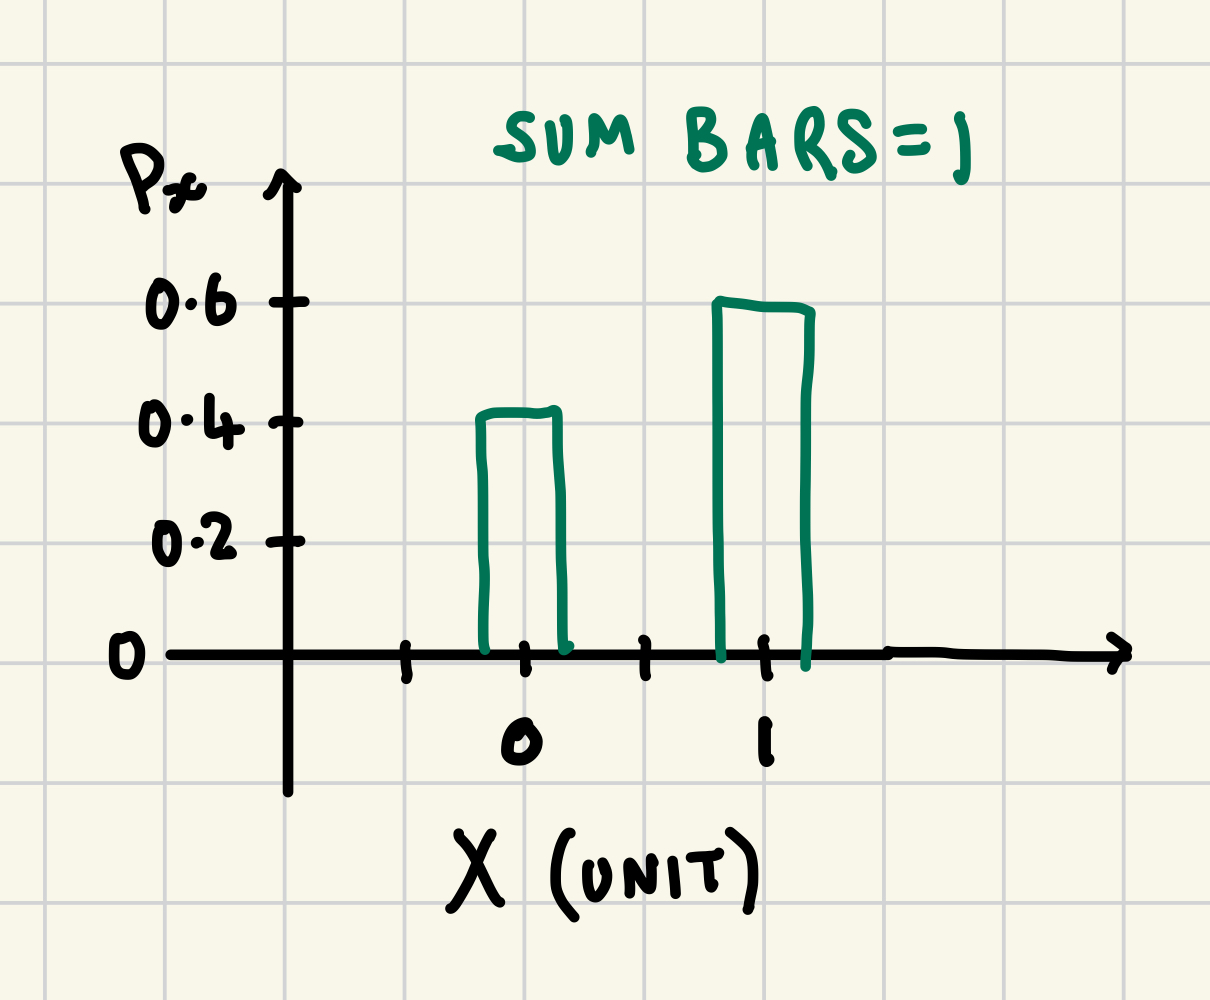
\includegraphics[scale=0.1]{bernoulli}

Our PMF is:\\
\small
\begin{equation}\nonumber
p_K(k) = 
\begin{cases}
     0\; & k<0\\[1ex] 
     1-p\; & k=0\\[1ex] 
  p\; & k=1 \\[2ex]
  0\; & k>1\\[2ex]
\end{cases}
\end{equation}

\end{multicols}
The support of K is all values k with non-zero probability: [0,1]. We write down the PMF for the support and for `outside the support' for completeness.\\[1ex]
\end{frame} 

\begin{frame}{Bernoulli PMF Plot }

\begin{center}
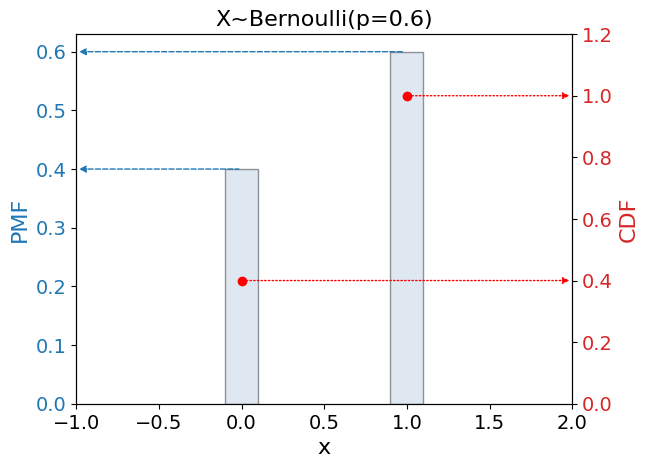
\includegraphics[scale=0.42]{Bern}
\end{center}

The CDF is not super helpful in this case, but will be useful later.
\end{frame} 



\begin{frame}{Bernoulli PMF: validity}

\small

Is $\sum\limits_{j_i \in S} p_K(k_i) =1$ ?\\[1ex]
\begin{equation}\nonumber
p_K(k) = 
\begin{cases}
     0\; & k<0\\[1ex] 
     1-p\; & k=0\\[1ex] 
  p\; & k=1 \\[2ex]
  0\; & k>1\\[2ex]
\end{cases}
\end{equation}

\vspace{0.5cm}

Normalisation check: $ \sum\limits_{k_i \in S} p_K(k_i) = p + (1-p) = 1$: the Bernoulli PMF is valid.

\end{frame} 


\begin{frame}{Bernoulli Probabilities}

The CDF $F_K(k) = P(K\leq k) = \sum\limits_{k_i}^{k} p_K(k_i) $ must be written in terms of ranges of values, because the Probability from the CDF is always for a range.\\

\begin{multicols}{2}
\small

\begin{equation}\nonumber
p_K(k) = 
\begin{cases}
     0\; & k<0\\[1ex] 
     1-p\; & k=0\\[1ex] 
  p\; & k=1 \\[2ex]
  0\; & k>1\\[2ex]
\end{cases}
\end{equation}

\begin{equation}\nonumber
F_K(k) = 
\begin{cases}
     0\; & k<0\\[1ex] 
  1-p\; & 0\leq k<1 \\[2ex]
  1\; & 1 \leq k \\[2ex]
\end{cases}
\end{equation}


\end{multicols}
\end{frame} 


\begin{frame}{Bernoulli: Expected Value \& Variance}

\boo{Expected Value}: \\[1ex]
$E[K]  = \sum\limits_{k_i \in S} k_i \,p_K(k_i)  = 0(1-p) + 1(p) = p$\\[1ex]

\boo{Variance}:\\[1ex]
$V[K]  =E[K^2]-E^2[K] $\\[1ex]
$E[K^2]  = \sum\limits_{k_i \in S} k^2_i p_K(k_i)  = 0^2(1-p) + 1^2(p) = p$\\[1ex]
$E^2[K] =p^2$\\[1ex]
$V[K]  = p-p^2 = p(1-p)$\\[1ex]

\end{frame} 

\begin{frame}[fragile]{Bernoulli: python}

\begin{minted}[bgcolor=LightGray]{python}
from scipy.stats import bernoulli
bernoulli.pmf(k, p, loc=0) 
\end{minted}
\vspace{0.5cm}

k is a number of successes, or user-provided array of values for the x-axis.\\[1ex]
p is the parameter: probability of success\\[1ex]
loc=0 is the default value of the location parameter, allowing for sliding along the x-axis if wanted. For example if for some reason you wanted success=6 and failure=5, you could set loc=5\\

\end{frame} 







\section{Binomial}

 
\begin{frame}{Binomial}
This time we will \boo{toss the coin n times}. I will count the number of heads, $k$, and that count is my Discrete RV $K$.\\[1ex]

$K\sim Binomial(n,p)$\\[1ex] 

The parameters are $n,p$ where $p$ is again the probability of (eg) success.\\[1ex]

Note that one Binomial trial consists of $n$ Bernoulli trials: Bernoulli was the number of heads from one toss.\\[1ex]

\end{frame} 


\begin{frame}{Binomial PMF}

The PMF is a bit of a mouthful:\\
\small
\begin{equation}\nonumber
p_K(k) = 
\begin{cases}
     0\; & k<0\\[1ex] 
     C_k^n\, p^k\, (1-p)^{n-k} \; & 0\leq k \leq n\\[1ex] 
 0 & k>n \\[2ex]
\end{cases}
\end{equation}

\end{frame} 

\begin{frame}{Binomial PMF plot}

%The distribution looks like this for $p=0.5$:\\
\centering
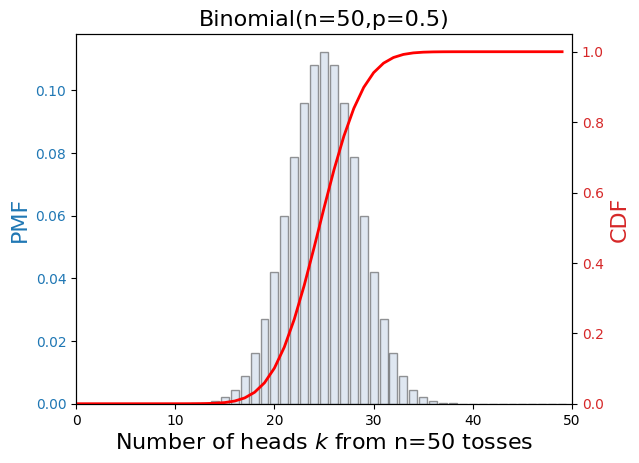
\includegraphics[scale=0.45]{BinomCoin.png}

\footnotesize

\boo{This is theory, not data. To generate this distribution with actual coin tosses you would get one data point for each set of 50 tosses. Then you could repeat it maybe a thousand times to get a distribution something like this.}

\end{frame} 



\begin{frame}{Binomial PMF dissected}

$p_K(k) = \textcolor{red}{C_k^n} \textcolor{blue}{p^k}\textcolor{purr}{ (1-p)^{n-k}}$ for $0\leq k \leq n$\\[2ex]

\small

\textcolor{blue}{$p^k$: probability of heads, $p$, to the power of the number of  heads observed, $k$}\\[1ex]

\textcolor{purr}{ $(1-p)^{n-k}$: probability of not heads, $1-p$, to the power of the number of not-heads observed, $n-k$.}\\[1ex]

$\textcolor{red}{C_k^n}$ is called the binomial coefficient. We need it because we are counting the number of heads, and \textbf{there is more than one way to get $k$ heads from $n$ tosses}. For example if $n=4$ and $k=3$ we have:\\[1ex]

HHHT, HHTH, HTHH, THHH: four different ways: $\textcolor{red}{C_k^n} =4$.\\[1ex]
\end{frame} 


\begin{frame}{Binomial Coefficient}

$\textcolor{red}{C_k^n} = n! /k!(n-k)!$ : (N combinations) / (N successful )(N unsuccessful)\\[1ex]

%The factorial $n!$ means $n(n-1)(n-2)...$\\[1ex]

For example, $C_k^n = 4!/3!(4-3)! = 4\cdot 3\cdot 2\cdot 1/ [(3\cdot 2 \cdot 1)\cdot ( 1) ]= 4$\\[1ex]

Factorials:\\
\begin{multicols}{2}
\small
$4! =4\cdot 3\cdot 2\cdot 1=24$\\[1ex]
$3! =3\cdot 2\cdot 1=6$\\[1ex]
$2! =2\cdot 1 =2$\\[1ex]
$1! = 1$\\[1ex]
\textbf{$0! =1$ by definition}\\[1ex]
\textbf{$-1!= NAN$ undefined}\\[1ex]
$\boo{a!/(a-1)! = a}$\\[1ex] %for example $4!/3! = 4$\\[1ex]

\end{multicols}

\end{frame} 


\begin{frame} [fragile] {Binomial Coefficients can be very large}
\small

$\textcolor{red}{C_k^n} = n! /k!(n-k)!$ : (N combinations) / (N successful )(N unsuccessful)\\[1ex]

Binomial coefficients can be \textbf{very large}.\\

$\boo{a!/(a-1)! = a}$: this is useful only when we have a single `failure'.\\

For example if we toss a coin 20 times and get 9 heads, the number of ways that can happen is:\\
\begin{minted}[bgcolor=LightGray]{python}
import math
# 20 tosses, 9 heads
math.factorial(20)/ ( math.factorial(9)*math.factorial(11) )
167_960
# 30 tosses, 15 heads
math.factorial(30)/ ( math.factorial(15)*math.factorial(15) )
155_117_520
\end{minted}






\end{frame} 





\begin{frame}{Binomial PMF: validity}

\small

$p_K(k) = \textcolor{red}{C_k^n} \textcolor{blue}{p^k}\textcolor{purr}{ (1-p)^{n-k}}$ for $0\leq k \leq n$\\[1ex]

Is $\sum\limits_{j_i \in S} p_K(k_i) =1$ ?\\[1ex]


There is no predefined limit on $n$, and $k$ can take any non-negative value up to  and including $n$: we have a sum to infinity. When that happens we need a SERIES. The series we need in this case is called the binomial series (or binomial theorem):\\[1ex]

$(a+b)^n = \sum\limits_{k=0}^{\infty} C_k^n \textcolor{blue}{a^k} \textcolor{purr}{b^{n-k}}$: we have $\textcolor{blue}{a=p}, \textcolor{purr}{b=1-p}$\\[1ex]


Normalisation check: $ \sum\limits_{k=0}^{\infty}  p_K(k_i) = (p+(1-p))^n =1^n = 1$: the Binomial PMF is valid.

\end{frame} 


\begin{frame}{Binomial Probabilities}

The Probability of $k \leq m$ successes is:\\[1ex]

 $P(K\leq m) = \sum\limits_{k=0}^{m} \textcolor{red}{C_k^n} \textcolor{blue}{p^k}\textcolor{purr}{ (1-p)^{n-k}}$ \\[1ex]
 
 \small
For example, the probability of tossing a coin n=5 times and getting \textbf{up to} k=4 heads on the toss of a fair coin with $p=0.5$ is:\\[1ex]
 
$P(K\leq 4) = \sum\limits_{k=0}^{4} \dfrac{ 5!}{ k!(5-k)!}\, 0.5^k 0.5^{5-k} = 0.96875$\\[1ex]

The probability of getting \textbf{at least} k=4 heads is calculated as:\\[1ex]

$1 - P(K\leq 3) =1 - \sum\limits_{k=0}^{3} \dfrac{ 5!}{ k!(5-k)!}\, 0.5^k 0.5^{5-k} = 0.1875$\\[1ex]
 
 

\end{frame} 


\begin{frame}{Binomial: Expected Value}

\boo{Expected Value}: \\[1ex]
$E[K]  = \sum\limits_{k_i \in S} k_i \,p_K(k_i)$\\[1ex]

Note that the total number of successes $k =  \sum k_i$, so we can write:\\[1ex]

$E[K] = E\left[\sum\limits_{k_i \in S} k_i\right] = \sum\limits_{k_i \in S} E[k_i]$\\[1ex]

\blu{The expectation of a sum is the sum of expectations:$E[X+Y] = E[X]+E[Y]$}\\[1ex]

$E[k_i]$ is the probability of success, $p$. So  \textbf{$E[K] =  \sum\limits_{0}^{n} p = np$}

\end{frame} 

\begin{frame}{Binomial: Variance}
\boo{Variance}:\\[1ex]
$V[K]  =E[K^2]-E^2[K] $: for once we will not use this form, as it is a long road.\\[1ex]

Because Binomial is $n$ repeated Bernoulli trials, we can extract the variance directly from $Bernoulli\; V[K]  = p(1-p)$.\\[1ex]

$\textbf{Binomial\; V[K] = np(1-p)}$.\\[1ex]

The variance of a sum of \boo{independent} experiments is the sum of the variance of each of them. V[sum] = sum[V ]\\[1ex]
%Recall the alternative form for variance $V[X]  =E[ ( X - E[X] )^2] $: Variance is an expectation.\\[1ex]

%We already stated that the $E[sum] = sum E$ (true even if X,Y not independent)\\[1ex]
 
\end{frame}


\begin{frame}[fragile]{Binomial: python}

\begin{minted}[bgcolor=LightGray]{python}
from scipy.stats import binom
binom.pmf(k, n, p, loc=0)
\end{minted}

\vspace{0.5cm}

k is number of successes, or user-provided array of values for the x-axis.\\[1ex]
n is the parameter: number of trials\\[1ex]
p is the parameter: probability\\[1ex]
loc=0 is the location parameter\\

\end{frame} 


%\section{Geometric}
%
%\begin{frame}{Geometric}
%
%\end{frame} 
%
%\begin{frame}{Geometric PMF}
%
%\end{frame} 
%
%\begin{frame}{Geometric PMF Plot}
%
%\end{frame} 
%
%\begin{frame}{Geometric PMF Validity}
%
%\end{frame} 
%
%\begin{frame}{Geometric Probabilities}
%
%\end{frame} 
%
%\begin{frame}{Geometric Variance \& Expectation}
%
%\end{frame} 
%
%\begin{frame}{Geometric  PMF: python}
%
%\end{frame}



\section{Poisson}


\begin{frame}{Poisson}
We don't just want to model coin flips. Something very important to humans is time. What is the count of `successful' outcomes \textbf{in a given time period}?\\[1ex]

$K\sim Poisson(\lambda)$\\[1ex] 

The parameter is $\lambda$: the success rate.\\[1ex]


\end{frame} 


\begin{frame}{Poisson PMF}

The Poisson PMF is:  $p_K(k) =  e^{-\lambda}\, \dfrac{ \lambda^k}{k!}$   for $k>= 0$ \\[1ex]

$k$ is the count of successful outcomes (our RV) in a fixed period of time.\\[2ex]
$\lambda$ is the success rate: a parameter of the distribution\\[2ex]
$ e^{-\lambda} = \exp{-\lambda}$: $e$ is Euler's number.\\[2ex]

\end{frame} 


\begin{frame}{Poisson PMF plot}

\centering
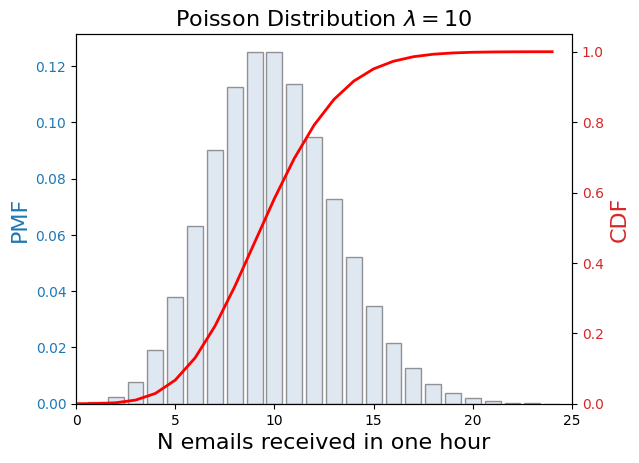
\includegraphics[scale=0.5]{PoissonExample.png}
\end{frame} 


\begin{frame}{Poisson PMF: validity}

Is  $ \sum\limits_{n=0}^{\infty} e^{-\lambda} \dfrac{ \lambda^k}{k!} =1$?\\[1ex]


\blu{For this PMF we again have an infinite range for our RV. When that happens we need a SERIES. We can look up the exponential series}:\\[1ex]
$e^{x} =\sum\limits_{x=0}^{\infty}  \dfrac{x^n}{n!} $: good for us with $x\rightarrow \lambda$ and $n\rightarrow k$\\[1ex]

 $e^{-\lambda} \sum\limits_{k=0}^{\infty}\dfrac{ \lambda^k}{k!} = e^{-\lambda} e^{\lambda}  = e^{-\lambda+\lambda}  =e^{0} =1$ because $e$ is a number.\\[1ex]

Normalisation check: the Poisson PMF is valid.

\end{frame} 


\begin{frame}{Poisson Probabilities}

The CDF is as usual: $P(K\leq k) = F_K(k) = \sum\limits_{k_i=0}^{k} p_K(k_i) $\\

The PMF is $p_K(k) =  e^{-\lambda} \dfrac{ \lambda^k}{k!}$   for $k>= 0$ \\[1ex]
 
\blu{I receive $\lambda \approx 100$ emails per 10-hour day. What is the probability of me getting zero emails in a given hour?}\\[1ex]

$\lambda  = 10$ is the rate per hour.\\[1ex]

$P(K=0) = F_K(0) =  e^{-10} \dfrac{ 10^0}{0!} = e^{-10} \dfrac{ 1}{1} \approx 4.5\times 10^{-5} $\\[1ex]
 

\end{frame} 


\begin{frame}{Poisson: Expected Value}

%$p_K(k) =  e^{-\lambda} \dfrac{ \lambda^k}{k!}$   for $k>= 0$
\small

\boo{Expected Value}: \\[1ex]
$E[K]  = \sum\limits_{k_i =0}^{\infty} k_i \,p_K(k_i) = \sum\limits_{k_i =0}^{\infty} k_i\, e^{-\lambda} \dfrac{ \lambda^{k_i}}{k_i!}$\\[1ex]

\boo{I want to use the exponential series to make this sum manageable.} $e^x = \sum\limits_{n=0}^{\infty} \dfrac{x^n}{n!}$\\[1ex]

It is going to need massaging into shape to have the right form.\\[1ex]

%\blu{Note 1: the $k=0$ term is zero.}\\[1ex]
\blu{Note:  $\dfrac{k}{k!} = \dfrac{1}{(k-1)!}$}\\[1ex]
\blu{Also:  $\lambda^{k} =\lambda^{k-1+1}  =\lambda^{k-1}\lambda $} \\[1ex]

\end{frame} 




\begin{frame}{Poisson: Expected Value}

%$p_K(k) =  e^{-\lambda} \dfrac{ \lambda^k}{k!}$   for $k>= 0$
\small

\boo{Expected Value}: \\[1ex]
$E[K]  = \sum\limits_{k_i =0}^{\infty} k_i \,p_K(k_i) = \sum\limits_{k_i =0}^{\infty} k_i\, e^{-\lambda} \dfrac{ \lambda^{k_i}}{k_i!}$\\[1ex]
\blu{Note 2:  $\dfrac{k}{k!} = \dfrac{1}{(k-1)!}$ and $\lambda^{k} =\lambda^{k-1+1}  =\lambda^{k-1}\lambda $} \\[1ex]

$E[K]  = e^{-\lambda} \sum\limits_{k_i =0}^{\infty}  \dfrac{ \lambda^{k_i}}{(k_i-1)!} =  \lambda e^{-\lambda} \sum\limits_{k_i =0}^{\infty}  \dfrac{ \lambda^{k_i-1}}{(k_i-1)!} $\\[1ex]


%$E[K]  = e^{-\lambda} \sum\limits_{k_i =1}^{\infty}  \dfrac{ \lambda^{k_i}}{(k_i-1)!} =  \lambda e^{-\lambda} \sum\limits_{k_i =1}^{\infty}  \dfrac{ \lambda^{k_i-1}}{(k_i-1)!} $\\[1ex]

Now we see we can use the exponential series again: \\[1ex]
$e^{x} = \sum\limits_{n=0}^{\infty} \dfrac{x^n}{n!} $: good for us with $x\rightarrow \lambda$ and $n\rightarrow k-1$\\[1ex]

\textbf{$E[K] = \lambda e^{-\lambda}  e^{\lambda} =\lambda $}: \boo{which makes sense}.\\[1ex]
\blu{Note: its okay that we have the $n\rightarrow k-1$ in the sum, because the $k=0$ term is zero.}\\[1ex]
\end{frame} 





\begin{frame}{Poisson: Variance}

\boo{Variance}:\\[1ex]
\textbf{$ V[K]  =E[K^2]-E^2[K] =\lambda$}\\[1ex]

OPTIONAL! Proof of this is a little bit fiddly but not too long. Give it a go, or/and see proof here: \href{https://proofwiki.org/wiki/Variance_of_Poisson_Distribution}{proofwiki}.\\[1ex]

Don't \cancel{waste} spend time trying this unless everything we are doing is a total cake-walk, and you are an expert at python, and you know how to make beautiful plots.\\[1ex]
\end{frame} 


\begin{frame}[fragile]{Poisson: python}

\begin{minted}[bgcolor=LightGray]{python}
from scipy.stats import poisson
poisson.pmf(k, mu, loc=0)
\end{minted}
\vspace{0.5cm}

k is a number per time period, or user-provided array of values for the x-axis.\\[1ex]
mu is the parameter we have called $\lambda$. This makes sense because the expected value $E[K]  =\lambda$, and we use the notation $E[K] \equiv \mu$.\\[1ex]
loc=0 is the location parameter\\

\footnotesize
\boo{Note: lambda has a special meaning in python, so is never used for a parameter name.}

\end{frame} 


\begin{frame}{Poisson versus Binomial}
\small

My friend Alf owns a donut shop in Brighton. On average, he sells 17.4 donuts a day (he is only open between 09:30 and 10:30).\\[1ex]
\blu{How should he model the number of donuts he sells as an RV?}\\[1ex]

\centering

\includegraphics[scale=0.5]{donut}

\end{frame} 


\begin{frame}{Poisson versus Binomial}
\small

My friend Alf owns a donut shop in Brighton. On average, he sells 17.4 donuts a day (he is only open between 09:30 and 10:30).\\[1ex]
\blu{How should he model the number of donuts he sells as an RV?}\\[1ex]

\begin{columns}
\begin{column}{0.5\textwidth}

The obvious choice is to go with  $X\sim\; Poisson(\lambda=17.4)$.\\[2ex]
\blu{A less obvious choice would be to go with $X\sim\; Binomial(n,p)$: n is the number of people in Brighton, p is the probability that any of them buys a donut.}\\[1ex]

\end{column}
\begin{column}{0.5\textwidth}


\includegraphics[scale=0.5]{donut}

\end{column}
\end{columns}



\end{frame} 



\begin{frame}[fragile]{Poisson versus Binomial}
\small
\begin{columns}
\begin{column}{0.5\textwidth}

Comparing the expectations, Poisson $E[K] = \lambda$, Binomial $E[K] = np$. So $\lambda = np$ or $p=\lambda/n$.\\[2ex]
In the limit of $n\to \infty$, the Binomial is a valid model. Note that the rate $\lambda$ has no limit on the number of people it draws from.\\[2ex]


\end{column}
\begin{column}{0.5\textwidth}


\includegraphics[scale=0.5]{donut}

\end{column}
\end{columns}

\boo{In the limit of $n\to \infty$,  $Binomial(n, \lambda/n) \rightarrow Poisson(\lambda)$} \\[1ex]
\end{frame} 



\begin{frame}[fragile]{Alf's donut shop}

Alf concludes that it is safer to use $X\sim Poisson(\lambda)$ as his model for donut sales.\\[2ex]

\centering
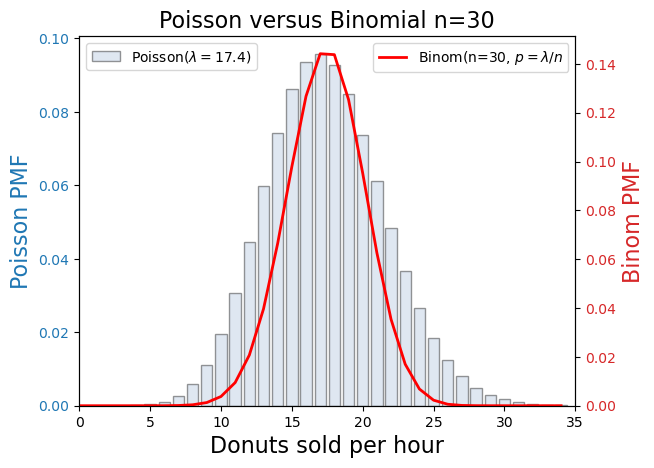
\includegraphics[scale=0.35]{Poissonbinom30.png}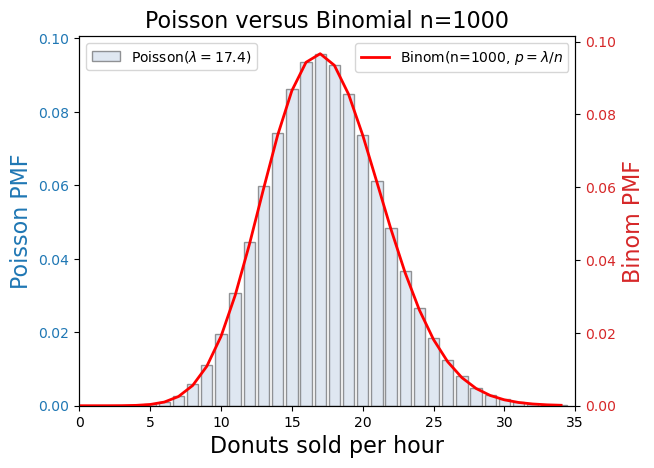
\includegraphics[scale=0.35]{Poissonbinom1k.png}

\end{frame} 

\begin{frame}{}
\Large
\centering
Now: Special PDFs (continuous RVs)

\end{frame} 


\section{Uniform}

\begin{frame}{Uniform}

The uniform pdf is flat between the lower and upper bound, and zero elsewhere.\\[1ex]

$X\sim Uniform(a,b)$\\[1ex] 

The parameters are $a,b$: the upper and lower bounds of the support.\\[1ex]

\end{frame} 

\begin{frame}{Uniform PDF}

We can write the PDF:\\[1ex]

\small
\begin{equation}\nonumber
f_X(x) = 
\begin{cases}
     constant\; & a<= x<=b\\[1ex] 
      0 & elsewhere \\[2ex]
\end{cases}
\end{equation}


\end{frame} 

\begin{frame}[fragile]{Uniform PDF Plot}

\begin{center}
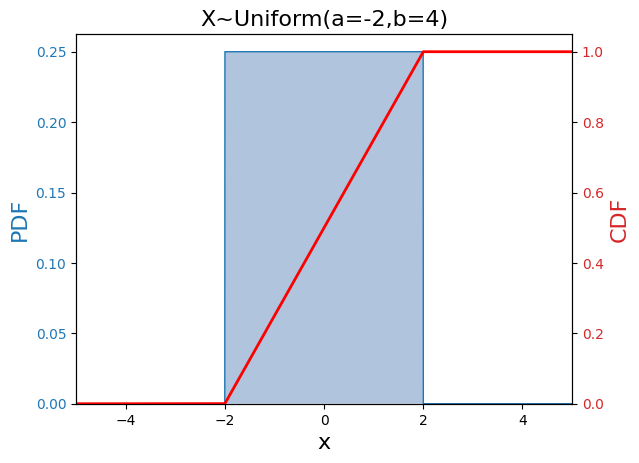
\includegraphics[scale=0.45]{Uniform.png}
\end{center}
\small
\boo{Note! the values on the y-axis are meaningless for PDFs. Cannot read off individual probabilities like we can for PMFs.}
\end{frame} 


\begin{frame}{Uniform PDF: validity}

We have so far only defined the PDF as $f_X(x) =c$ for $a<= x<=b$, so this is very easy.\\[1ex]

$\int\limits_a^b c\, dx = c\,x \bigg|_a^b = c(b-a) =1$, so $c = \dfrac{1}{ b-a}$\\[1ex]

Normalisation check \textit{gives us the form} $f_X(x) =\dfrac{1}{ b-a}$  for $ a\leq x\leq b$\\[1ex]

The Uniform PDF is valid.

\end{frame}  

\begin{frame}{Uniform Probabilities}

Recall that we can \textit{only} use the CDF (not the PDF) for probabilities associated with CRVs.\\[1ex]

$P(X\leq x) = F_X(x) = \displaystyle \int_a^x \dfrac{1}{ b-a} dx = \dfrac{x}{ b-a} \bigg|_a^x =  \dfrac{x-a}{ b-a} $\\[1ex]

\small
\begin{equation}\nonumber
F_X(x) = 
\begin{cases}
     0\; & x<a\\[1ex] 
     \dfrac{x-a}{ b-a} & a<= x<=b\\[1ex] 
      1 & x>b \\[2ex]
\end{cases}
\end{equation}

\end{frame}  

\begin{frame}{Uniform PDF Expected Value \& Variance}
\small

\boo{Expected Value:}\\[1ex]

$E[X]  = \int\limits_{a}^{b} x\, f_X dx = \int\limits_{a}^{b}  \dfrac{x}{b-a}\, dx = \dfrac{x^2}{2(b-a)}\bigg|_a^b = \dfrac{b^2-a^2}{2(b-a)} = \dfrac{ (b+a)}{2}$\\[1ex]

\boo{Variance:}\\[1ex]

$V[X]  =E[X^2] - E^2[X]$\\[1ex]
$E^2[X]  = \dfrac{ (b+a)^2}{4}$\\[1ex]
$E[X^2]  = \int\limits_{a}^{b} \dfrac{x^2}{b-a}\, dx =  \dfrac{b^3-a^3 }{3(b-a)}$\\[1ex]
$V[X]   = \dfrac{b^3-a^3 }{ 3(b-a)} - \dfrac{ (b+a)^2}{4} = \dfrac{ (b-a)^2}{12}$ \blu{optional algebra exercise: prove this.}\\[1ex]

\end{frame}  

\begin{frame}[fragile]{Uniform PDF: python}

\begin{minted}[bgcolor=LightGray]{python}
from scipy.stats import uniform
uniform.pdf(x, loc=0, scale=1)
\end{minted}
\vspace{0.5cm}

x is a user-provided range of values for the x-axis.\\[2ex]
loc=0 is the location parameter. For us this is loc=a\\[2ex]
scale=1 is the scale parameter. For us this is scale=b-a\\[2ex]

\end{frame} 



\section{Exponential}

\begin{frame}{Exponential}

The exponential distribution is essentially a 'waiting times' distribution.\\[1ex]

$T\sim Expon(\lambda)$\\[2ex]

\blu{I am using $X\rightarrow T$ for the single RV because I want us to be really clear that this is time. I am a physicist...}

\end{frame} 

\begin{frame}{Exponential PDF}
$f_T(t) = \lambda e^{-\lambda t} $ for $0\leq t \leq \infty$\\[1ex]

Compare with the Poisson PDF which models $K$ : counts in a given time.\\[1ex]

Recall, $K \sim Poisson(\lambda): p_K(k) = \dfrac{\lambda^{k}}{k!} e^{-\lambda}$\\[1ex]

In both cases we have $\lambda = events/time$ but \blu{for Poisson our expectation is a count for fixed time}, and we shall see that \boo{for Expon the expectation is a time for fixed counts}.\\[1ex]

\end{frame} 

\begin{frame}{Exponential PDF Plot}


\begin{center}
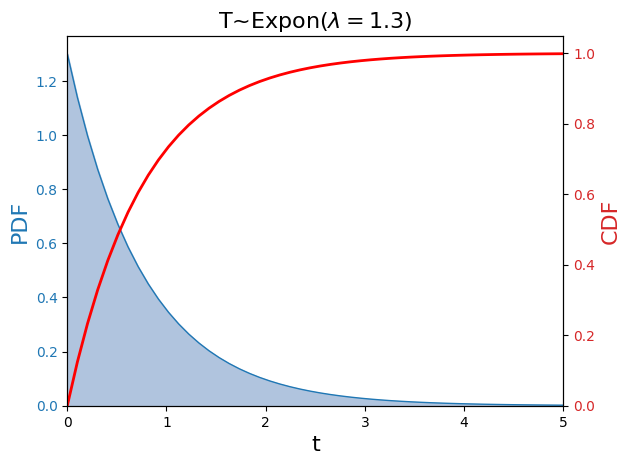
\includegraphics[scale=0.4]{Expon.png}
\end{center}

\footnotesize
It may not look like it, but the CDF does not  actually reach 1 until $t=\infty$.\\
\end{frame} 

\begin{frame}{Exponential PDF Validity}

Is $ \int\limits_0^\infty \lambda e^{-\lambda t} dt =1$?\\[1ex]

$\int\limits_0^\infty \lambda e^{-\lambda t} dt  =  -\dfrac{\lambda }{\lambda} e^{-\lambda t} \bigg|_0^{\infty} = - [ e^{-\infty}- e^{0}] = -[0-1]=1$\\[1ex]

The Exponential PDF is valid for $0\leq t \leq \infty$.

\end{frame} 

\begin{frame}{Exponential Probabilities}

\small

$P(T\leq t) = F_T(t) = \displaystyle \int_{0}^t  \lambda e^{-\lambda t} \,dt = - [e^{-\lambda t} - e^{0}] = 1 - e^{-\lambda t} $\\[1ex]

I can use this to figure out the probability for example that I will wait less than or equal to one hour to hitch a lift on a road with an average rate of hitch-hiker pickups of $\lambda=1.3$ per hour.\\[1ex]

$P(T\leq 1H) =  1 - e^{-1.3} = 0.727$\\[1ex]

\blu{What would Poisson give us? Now we are asking the question: `what is the probability that a count of not zero occurs in a time period of 1H?'}\\[1ex] 

$p_K(k=0) =  e^{-1.3} \dfrac{ 1.3^0}{0!}  = e^{-1.3} = 0.273$ : probability of zero pickups.\\[1ex]

Probability of `not zero' in 1H is $1-e^{-1.3}= 0.727$ as before.\\[1ex]

\end{frame}



\begin{frame}{Exponential Expected Value}

\boo{Expected Value:}\\[1ex]

$E[T]  = \int\limits_0^{\infty} t\, f_T\, dt = \int\limits_0^{\infty} t\, \lambda e^{-\lambda t} \, dt $\\[1ex]


\blu{This integral is a product of two terms in t, so we have to do it piecewise (integration by parts). This is an excellent exercise, try it if you have time.}\\[1ex]

I did: $u =t$, $u'=1$, $v = -e^{-\lambda t}$, $v'= \lambda e^{-\lambda t}$\\[1ex]

You will find $\mathbf{E[T]  = \dfrac{1}{\lambda}}$\\[1ex]

\end{frame} 


\begin{frame}{Exponential Variance}

\boo{Variance:}\\[1ex]

$V[T]  =E[T^2] - E^2[T]$\\[1ex]

I found this needed two rounds of integration by parts, but perhaps it could be done in one round I think. Let me know!\\[1ex]

You will find: $\mathbf{V[T] = \dfrac{1}{\lambda^2}}$

\end{frame} 



\begin{frame}[fragile]{Exponential PDF: python}

\begin{minted}[bgcolor=LightGray]{python}
from scipy.stats import expon
expon.pdf(x, loc=0, scale=1)
\end{minted}

\vspace{0.5cm}

x is a user-provided range of (time) values for the x-axis.\\[2ex]
loc=0 is the location parameter.\\[2ex]
scale=1 is the scale parameter. The scale is 1/rate=$1/\lambda$).\\[2ex]

\end{frame}

\begin{frame}[fragile]{Exponential PDF is \boo{Memoryless} }
You are waiting for a taxi. The average number of taxis per minute is $\lambda$.\\[1ex]

The probability of a taxi arriving in the first $n$ mins is $p=P(T\leq n)$.\\[1ex]

A taxi does not arrive in the first five mins :(. The probability of it arriving in the next five mins is still $p$. \\[1ex]

This is annoying! But it is not a paradox. \\[1ex]

\end{frame}


\begin{frame}[fragile]{Exponential PDF is \boo{Memoryless}}
\small
Let $A = T\geq  t+n $ and $B = T \geq n$. Note that $B\subset A$.\\[2ex]
\blu{This means that A is the event where the wait is longer than t+n. This event A entirely contains the event where the wait is longer than t, for all non-negative values of n.}\\[1ex]

Let's remind ourselves of the exponential PDF and CDF:\\[1ex]
$f_T(t) = \lambda e^{-\lambda t} $ for $0\leq t \leq \infty$\\[1ex]
$P($\blu{$T\leq t$}$) = F_T(t) = \displaystyle \int_{0}^t  \lambda e^{-\lambda t} \,dt = - [e^{-\lambda t} - e^{0}] = 1 - e^{-\lambda t} $\\[1ex]
$P($\blu{$T\geq t$}$) = 1 - F_T(t) =  e^{-\lambda t} $\\[1ex]

\blu{We are not double counting $t=0$, because $P(t=0) = 0$ for a CRV.}\\

$P(A) \equiv P(T \geq t+n) = 1-P(T \leq t+n) = e^{-\lambda(t+n)}$.\\[1ex]
$P(B) \equiv P(T \geq n) = 1-P(T \leq n) = e^{-\lambda(n)}$.\\[1ex]




%Conditional probability $P(A|B) = \dfrac{P(A\cap B)}{P(B)} = \dfrac{P(A)}{P(B)}$  because $B\subset A$.\\[3ex]
%$P(A|B)  = e^{-\lambda(t+n)} / e^{-\lambda n} = e^{-\lambda(t+n-n)} = e^{-\lambda t}. $\\[3ex]
%\blu{What this tells us is the probability of our new waiting time is independent of the time we have already waited. Bah!}\\[2ex]

\end{frame}


\begin{frame}[fragile]{Exponential PDF is \boo{Memoryless}}
\small
Let $A = T\geq  t+n $ and $B = T \geq n$. Note that $B\subset A$.\\[2ex]
$P(A) \equiv P(T \geq t+n) = 1-P(T \leq t+n) = e^{-\lambda(t+n)}$.\\[2ex]
$P(B) \equiv P(T \geq n) = 1-P(T \leq n) = e^{-\lambda(n)}$.\\[2ex]
Conditional probability $P(A|B) = \dfrac{P(A\cap B)}{P(B)} = \dfrac{P(A)}{P(B)}$  because $B\subset A$.\\[3ex]
$P(A|B)  = e^{-\lambda(t+n)} / e^{-\lambda n} = e^{-\lambda(t+n-n)} = e^{-\lambda t}. $\\[3ex]
\blu{What this tells us is the probability of our new waiting time is independent of the time we have already waited. Bah!}\\[2ex]

\end{frame}


\section{Beta}

\begin{frame}{Beta}

The Beta distribution is a gem when it comes to defining \boo{prior probability distributions} $\pi(\theta)$.\\[1ex]

$X \sim Beta(\alpha,\beta)$\\[2ex]

We shall see that the reason for its special usefulness is that it is constructed such that we can decide its (hyper) parameters $\alpha, \beta$ based on the expectation and variance we seek, while having a distribution that is a chameleon in terms of its shape.\\[1ex]

\end{frame} 


\begin{frame}{Beta PDF}

\small

$f_X(x) = \dfrac{1}{B(\alpha,\beta)}\, x^{\alpha-1} (1-x)^{\beta-1}$, for $0\leq x \leq 1$, $\alpha>0$, $\beta>0$\\[1ex]

The limits on the RV: $0\leq x \leq 1$: \boo{we can use this when the RV is itself a probability}.\\[1ex]

If we don't know exactly what the probability is, but have some idea of the expectation and variance, we can use the Beta distribution .\\[1ex]

Normalisation factor:  $\dfrac{1}{B(\alpha,\beta)} = \dfrac{1}{ \int\limits_0^1 x^{a-1} (1-x)^{b-1} dx}$.\\[1ex]

\end{frame} 



\begin{frame}{Beta PDF Plots: The Chameleon!}

\centering
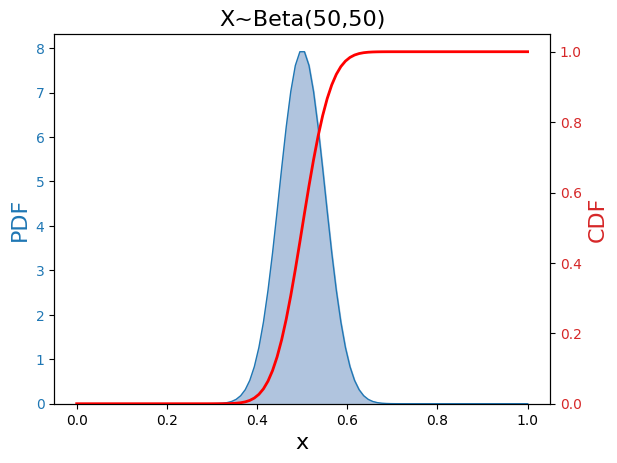
\includegraphics[scale=0.3]{Beta5050.png}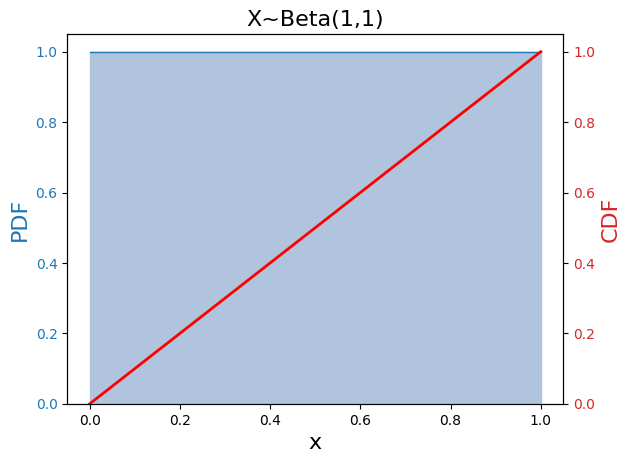
\includegraphics[scale=0.3]{Beta11.png}
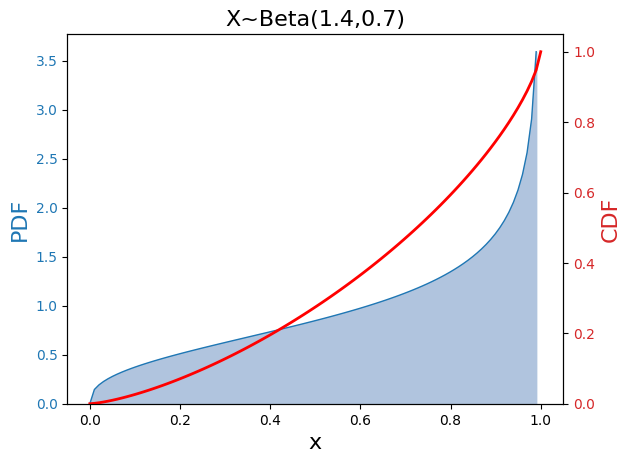
\includegraphics[scale=0.3]{Beta1407.png}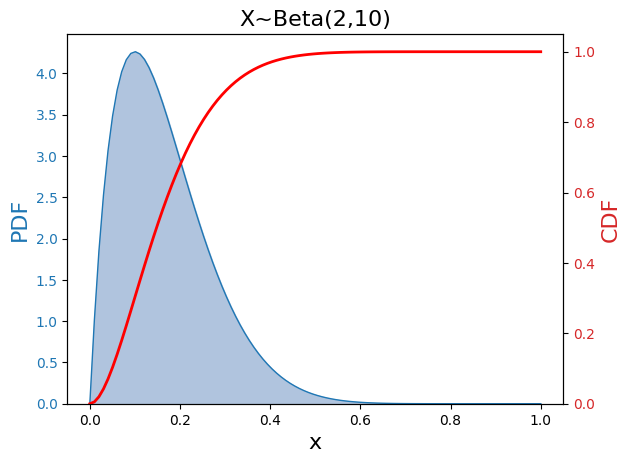
\includegraphics[scale=0.3]{Beta0210.png}



\end{frame} 


\begin{frame}{Beta Variance \& Expectation}

Integrating the Beta PDF is a bit too much like hard work for me, but I trust my sources for these:\\[3ex]
%For now we will just state the expectation and variance because they are a bit of a pain to get out (you dont need that for this).
 $E[X] = \int\limits_{0}^{1} x\, f_X dx =  \dfrac{\alpha}{\alpha + \beta}$\\[1ex] 
$V[X] = E[X^2] - E^2[X] = \dfrac{E[X](1-E[X])}{ \alpha+\beta+1} = \dfrac{\alpha \beta}{(\alpha + \beta)^2 (\alpha+\beta+1)} $\\[3ex]
\vspace{0.5cm}

%Variance depends on absolute value of  a+b
%plots of Beta(a,b) with a+b=constant show symmetry for a=b and different skews as we change the ratio a>b and b>a
%Expectation depends on relative value  a/a+b
%plots of Beta(a,b) with a/b=constant get peakier with smaller values.
I recommend (again?) looking at the \href{https://www.acsu.buffalo.edu/~adamcunn/probability/beta.html}{Probability Playground}.
\end{frame} 

\begin{frame}[fragile]{Beta PDF: python}

\begin{minted}[bgcolor=LightGray]{python}
from scipy.stats import beta
beta.pdf(x, a, b, loc=0, scale=1)
\end{minted}
\vspace{0.5cm}

x is a user-provided range of values (eg probabilities) for the x-axis.\\[1ex]
a = the Beta shape parameter $\alpha$. \\[1ex]
b= the Beta shape parameter $\beta$. \\[1ex]
loc=0 is the location parameter. \\[1ex]
scale=1 is the scale parameter\\[1ex]

\end{frame}

\begin{frame}{Beta PDF Example}
\small

We do not know if a coin is fair (hypothesis $p=0.5$) but we are studying it. We would like to generate a prior pdf with $E[X] =0.5$ and standard deviation $\sigma=\sqrt{V[X]}=0.1$. We can use a Beta distribution!\\[2ex]
Want $E[X] = 0.5$, so $E[X] = \dfrac{\alpha}{\alpha+\beta}$ means we must have $\alpha=\beta$.\\[2ex]
Want $V[X] = 0.1^2$, so $V[X]  = \dfrac{0.5(1-0.5) }{ \alpha+\beta+1} = \dfrac{0.25}{2\alpha+1} \therefore \alpha=12 (=\beta)$\\[2ex]
We will use $\pi(\theta) =  Beta(12,12) =  \dfrac{1}{B(a,b) }x^{11}\, (1-x)^{11}$\\[2ex]
\blu{When we look at this again later you will see how useful it is for Bayesian stats, but this is just a taster for now.}\\[1ex]
\end{frame}



\section{Normal}

\begin{frame}{Normal aka Gaussian}
The Normal distribution is the \boo{Queen Of Them All}.\\[1ex]

$X \sim Norm(\mu, \sigma)$\\[2ex]

Notice that the parameters are $\mu$, $\sigma$: these are the symbols we use to express the expectation and standard deviation of any distribution. \\[1ex]

\end{frame} 

\begin{frame}{Normal  PDF}


$f_X(x) = \frac{1}{\sigma \sqrt{2\pi}} e^{-\frac{1}{2} \frac{(x-\mu)^2}{\sigma^2}}$\\[1ex]

\vspace{0.5cm}

\normalsize
Often written in \boo{Standardised} form with $Z=\dfrac{X-\mu}{\sigma}$:\\[3ex]
\vspace{0.5cm}

$f_Z(z) = \frac{1}{\sigma \sqrt{2\pi}} e^{-\frac{1}{2} z^2}$\\[1ex]


\end{frame} 

\begin{frame}{Normal  PDF Plot}
\centering
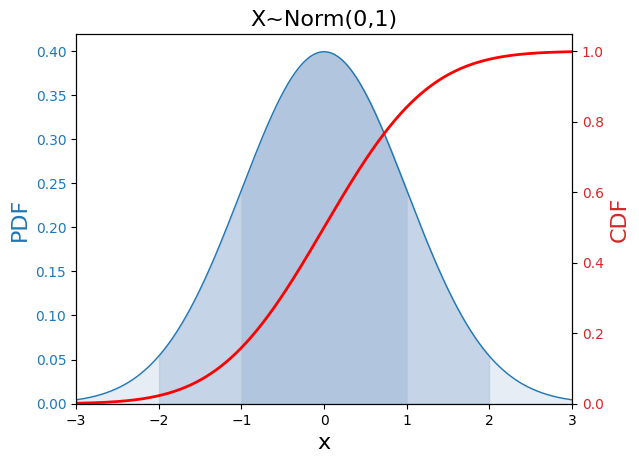
\includegraphics[scale=0.5]{Norm.png}
\end{frame} 

\begin{frame}{Normal  PDF Validity}

Is $\int\limits_{-\infty}^{\infty} f_X(x)\,dx =1$? Yes :) \\[1ex]


Integral is $\int\limits_{-\infty}^{\infty}  \frac{1}{\sqrt{2\pi}} e^{-\frac{x^2}{2}} dx$\\[1ex]

We can note the result: $\int\limits_{-\infty}^{\infty} e^{-x^2} dx = \sqrt{\pi}$\\[1ex]

See this super-clear proof from \href{https://www.youtube.com/watch?v=fWOGfzC3IeY}{Christine Breiner} (youtube).\\[1ex]

This gives us the normalisation factor of $\dfrac{1}{\sqrt{2\pi}}$ in the PDF.
\end{frame} 

\begin{frame}{Normal  Probabilities}
There is no analytical solution to the indefinite integral of the Gaussian PDF.\\[1ex]

Rather than calculating the CDF to get probabilities, we tend to look them up (some other kind soul did the approximations for  us and made lookup tables). I would use python, which does the same (error function) calculations used for the lookup tables.\\[1ex]

We can also use the very special properties of the Normal distribution to note down some useful probabilities.\\[1ex]

\end{frame} 


\begin{frame}{Normal  Probabilities}
\small

No matter what values of $\mu$ and $\sigma$, the normal distribution will always have $68\%, 95\%, 99.7\%$ of its area within $\pm 1,2,3$ standard deviations from the mean.\\[1ex]

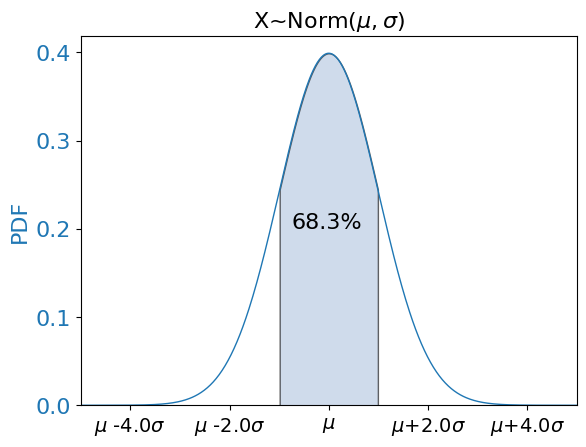
\includegraphics[scale=0.25]{Norm1sigma.png}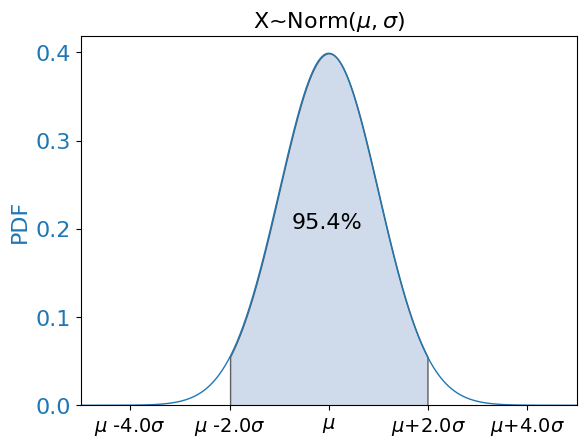
\includegraphics[scale=0.25]{Norm2sigma.png}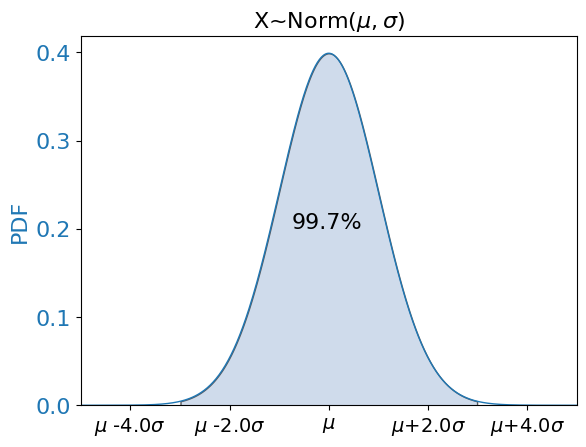
\includegraphics[scale=0.25]{Norm3sigma.png}
\vspace{0.5cm}

You would be forgiven for thinking that this distribution has its limits around $\pm 4\sigma$ from the mean. But the Normal distribution has limits of $\pm \infty$.\\

\end{frame} 

\begin{frame}{Particle Physicist's version}
\footnotesize
To see that the Gaussian distribution has tails (out to $\pm \infty$, but we can't plot that) we need to zoom on the lower part of the y-axis, which we can do by using a \boo{log scale}. We also need more significant figures. \blu{Particle physicists don't use the D-word unless we see something outside the $5\sigma$ range of probabilities, corresponding to a p-value of $5.7\times10^{-7}$ (a one in 5.7 million chance that it is a statistical fluctuation rather than an actual Discovery)}.

\centering
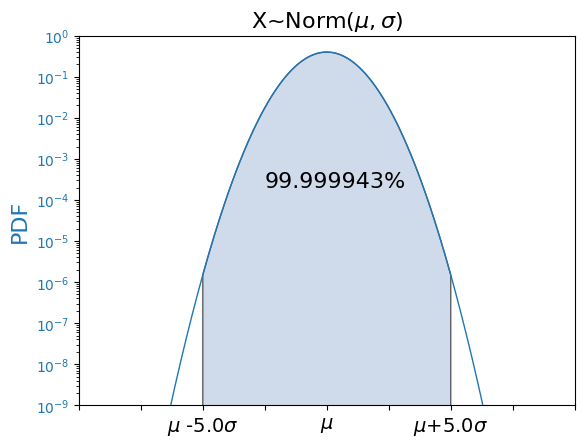
\includegraphics[scale=0.4]{Norm5sigmaLog.png}

\end{frame} 


\begin{frame}{Normal  Variance \& Expectation}

\blu{Breathe a sigh of relief, no crazy math needed!}\\[1ex]

The parameters of the Gaussian distribution are the expected value and standard deviation, so no work at all required here.\\[1ex]


Expected Value $\mathbf{E[X]  = \mu}$ \\[2ex]
Variance $\mathbf{V[X]  = \sigma^2}$ \\[2ex]


\blu{Note that this could seem like a tautology if we look at it the wrong way round. But it isn't.}\\[1ex]

\end{frame} 

\begin{frame}[fragile]{Normal PDF: python}

\begin{minted}[bgcolor=LightGray]{python}
from scipy.stats import norm
norm.pdf(x, loc=0, scale=1)
\end{minted}
\vspace{0.5cm}

x is a user-provided range of values for the x-axis.\\[2ex]
loc= $\mu = E[X]$\\[2ex]
scale= $\sigma = \sqrt{V[X]}$\\[2ex]

\end{frame}



\begin{frame}{Loads more coming on the Gaussian.}

If you thought it was weird that the $Binomial(n,p)$ is $Poisson(\lambda)$ in the limit of $n\rightarrow \infty$, just wait until you see what the Gaussian has up its sleeves.\\[1ex]

\vspace{0.5cm}

Before we go any further with the Gaussian, \boo{we need to talk about correlations and uncertainties}.\\[1ex]
\end{frame}



\begin{frame}{Thanks For Your Time}
\center
\Huge
Fin.
\end{frame}






\end{document}

 
 
 